\documentclass{article}[12pt]
\usepackage[utf8]{inputenc}
\usepackage[T1]{fontenc}
\usepackage[ngerman]{babel}
\usepackage[dvipsnames]{xcolor}
\usepackage{lipsum}

\usepackage{amsfonts}
\usepackage[intlimits]{amsmath}
\usepackage{cite}
\usepackage{epsfig}

\usepackage[usenames,dvipsnames]{pstricks}
\usepackage{pstricks-add}
\usepackage{epsfig}
\usepackage{pst-grad} % For gradients
\usepackage{pst-plot} % For axes

\addtolength{\hoffset}{-1.5cm}
\addtolength{\textwidth}{3cm}
\usepackage{listings}
\usepackage{color}
\definecolor{mygreen}{rgb}{0,0.6,0}
\definecolor{mygray}{rgb}{0.5,0.5,0.5}
\definecolor{mymauve}{rgb}{0.58,0,0.82}
\PassOptionsToPackage{svgnames}{xcolor}
\usepackage{tcolorbox}
\usepackage{lipsum}
\tcbuselibrary{skins,breakable}
\usetikzlibrary{shadings,shadows}

\lstset{ %
  backgroundcolor=\color{white},   % choose the background color; you must add \usepackage{color} or \usepackage{xcolor}; should come as last argument
  basicstyle=\footnotesize,        % the size of the fonts that are used for the code
  breakatwhitespace=false,         % sets if automatic breaks should only happen at whitespace
  breaklines=true,                 % sets automatic line breaking
  captionpos=b,                    % sets the caption-position to bottom
  commentstyle=\color{mygreen},    % comment style
  deletekeywords={...},            % if you want to delete keywords from the given language
  escapeinside={\%*}{*)},          % if you want to add LaTeX within your code
  extendedchars=true,              % lets you use non-ASCII characters; for 8-bits encodings only, does not work with UTF-8
  frame=single,                    % adds a frame around the code
  keepspaces=true,                 % keeps spaces in text, useful for keeping indentation of code (possibly needs columns=flexible)
  keywordstyle=\color{blue},       % keyword style
  language=C,                      % the language of the code
  morekeywords={*,...},            % if you want to add more keywords to the set
  numbers=left,                    % where to put the line-numbers; possible values are (none, left, right)
  numbersep=5pt,                   % how far the line-numbers are from the code
  numberstyle=\tiny\color{mygray}, % the style that is used for the line-numbers
  rulecolor=\color{black},         % if not set, the frame-color may be changed on line-breaks within not-black text (e.g. comments (green here))
  showspaces=false,                % show spaces everywhere adding particular underscores; it overrides 'showstringspaces'
  showstringspaces=false,          % underline spaces within strings only
  showtabs=false,                  % show tabs within strings adding particular underscores
  stepnumber=1,                    % the step between two line-numbers. If it's 1, each line will be numbered
  stringstyle=\color{mymauve},     % string literal style
  tabsize=2,                       % sets default tabsize to 2 spaces
  title=\lstname                   % show the filename of files included with \lstinputlisting; also try caption instead of title
}

\usepackage{amssymb}

\newenvironment{myexampleblock}[1]{%
    \tcolorbox[beamer,%
    noparskip,breakable,
    colback=White,colframe=ForestGreen,%
    colbacklower=LimeGreen!75!White,%
    title=#1]}%
    {\endtcolorbox}

\newenvironment{myalertblock}[1]{%
    \tcolorbox[beamer,%
    noparskip,breakable,
    colback=White,colframe=Bittersweet,%
    colbacklower=Peach!75!White,%
    title=#1]}%
    {\endtcolorbox}

\newenvironment{myblock}[1]{%
    \tcolorbox[beamer,%
    noparskip,breakable,
    colback=White,colframe=RoyalBlue,%
    colbacklower=TealBlue!75!White,%
    title=#1]}%
    {\endtcolorbox}

\newenvironment{myexampleprogram}[1]{%
    \tcolorbox[beamer,%
    noparskip,breakable,
    colback=White,colframe=Goldenrod,%
    colbacklower=Yellow!75!White,%
    title=#1]}%
    {\endtcolorbox}
%--------
%\usepackage[magyar]{babel}
\title{Zufallszahlengenerator}
\begin{document}
\maketitle
\noindent Zufällig generierte Zahlen sind ein wichtiges und mächtiges Werkzeug in der numerischen Physik. 
Sie finden beispielsweise zum Integrieren von Funktionen mit mehreren Variablen mit sogenannten Monte Carlo Verfahren Anwendung.

Allerdings sind die am Computer genutzten Zufallszahlen nicht tatsächlich zufällig, sondern sie werden durch einen deterministischen Algorithmus erzeugt. 
Deshalb spricht man von Pseudozufallszahlen.
In dieser Aufgabe werden wir einen Pseudozufallszahlengenerator schreiben. 
Dabei wird eine Reihe von Pseudozufallszahlen $I_0, I_1, I_2, \ldots$ erzeugt, die dann möglichst ähnlich zu einer Reihe echter Zufallszahlen ist.
Die Reihe wird beispielsweise mit folgender Iteration erzeugt:
\begin{equation}
  I_{j+1}=a I_{j} \left( \mathrm{mod}\ m\right)\,,\quad j=0,1,2,\ldots\,.
  \label{basics}
\end{equation}
Diesen Instruktion erstellt eine neue Zufallszahl ($I_{j+1}$) aus der vorangegangenen Zahl ($I_j$). Die Qualität der Zufallszahlen 
hängt von den Eingangsparametern $(a,m)$ ab. 
Ein guter Zufallszahlengenerator hat große Perioden, dass hei\ss{}t, es braucht sehr viele Iterationen in $j$ bis eine Zufallszahl $I_k$ erneut auftritt.
Die Periode ist deswegen so wichtig, weil sich die Reihe von da an exakt wiederholt.
Park und Miller haben die folgenden Parameter für $a$ und $m$ gewählt:
\begin{equation}
  a=16807\,,\quad m=2^{31}-1=2147483647\,. 
\end{equation}
Leider ist die direkte Implementation dieses Zufallszahlengenerators mit diesen Parametern in \texttt{C} mit dem Typ \texttt{int} nicht möglich. 
Der Grund ist, dass wir keine Zahlen größer als $m$ in einem \texttt{int} speichern können. 
(Mit Hilfe von \texttt{unsigned long int} kann man auf modernen Rechnern natürlich schon größere Zahlen darstellen, als $m$)
Glücklicherweise gibt es eine Möglichkeit das Problem algorithmisch umzugehen. 
Wir faktorisieren $m$ wie folgt:
\begin{equation}
  m = aq + r\,;\quad r= m \left(\mathrm{mod}\ a\right)\,;\quad q= \left[m/a\right]\,.
\end{equation}
Damit können wir die Gleichung (\ref{basics}) auch mit ($q,r$) darstellen:
\begin{equation}
  \begin{split}
    a I_j \left( \mathrm{mod}\ m\right)&=  
    (a\left(I_j \mathrm{mod}\ q\right) -r \left[I_j/q\right] + m)\ (\mathrm{mod}\ m)\\
    &=  \begin{cases}
      a\left(I_j \mathrm{mod}\ q\right) -r \left[I_j/q\right] & \mathrm{falls~}>0\,, \\ 
      a\left(I_j \mathrm{mod}\ q\right) -r \left[I_j/q\right] + m & \mathrm{sonst}\,. \\ 
    \end{cases}
  \end{split}
  \label{algo}
\end{equation}
Hierbei ist $r=2836$ und $q=127773$. 

Implementieren Sie den Zufallszahlengenerator nach Gleichung~\ref{algo}. 
Ändern Sie den Algorithmus so ab, dass er gleichverteilte Fließkommazahlen $u_j$ zwischen 0 und 1 erzeugt.
Um das Programm auf Korrektheit zu überprüfen, können wir beispielsweise die Verteilung der Zufallszahlen testen.
Da der Algorithmus gleichverteilte Zufallszahlen erzeugen soll, muss im Mittel jede reelle Zahl zwischen 0 und 1 gleichoft vorkommen.
Um das zu überprüfen, kann man ein Histogramm der erzeugten Zufallszahlen erzeugen.
Dafür unterteilt man das Interval $[0,1]$ in $n$ Abschnitte der Länge $\Delta=1/n$. 
Dann zählt man, wir viele Zufallszahlen $C_i$ im Interval $[x_i,x_i+\Delta]$ liegen, mit $x_i=i\Delta$ und $i=0,\ldots,n-1$.
Schließlich trägt man die Dichte $\rho(x_i)=C_i/N$ gegen $x_i$ auf, wobei $N$ die Gesamtzahl der gezogenen Zufallszahlen ist. 

Bespielsweise könnte man das Ergebnis graphisch wie folgt darstellen:
\begin{center}
  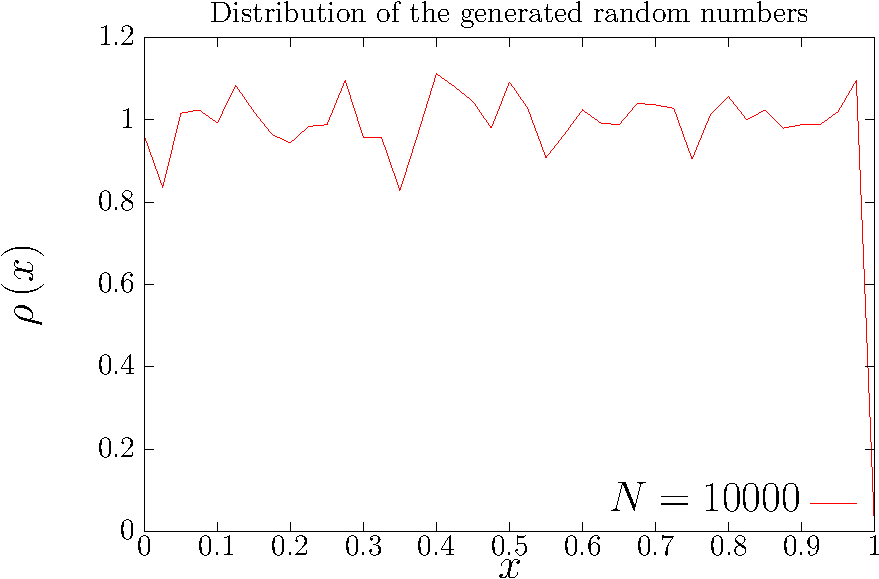
\includegraphics[width=.8\linewidth]{dist1.pdf}
\end{center}
Welchen Wert erwarten Sie für den Mittelwert 
\[
\bar x = \frac{1}{N}\sum_j u_j
\]
Ihrer Zufallszahlen?
Passt Ihre Erwartung zu Ihrer Implementation?

\end{document}
